
\documentclass[letterpaper,twocolumn,10pt]{article}
\usepackage{usenix-2020-09}

% to be able to draw some self-contained figs
\usepackage{tikz}
\usepackage{amsmath}

% inlined bib file
\usepackage{filecontents}


%-------------------------------------------------------------------------------
\begin{document}
%-------------------------------------------------------------------------------

%don't want date printed
\date{}

% make title bold and 14 pt font (Latex default is non-bold, 16 pt)
\title{\Large \bf IP Shuffle:\\
  Random IP Address Assignment for Network Interfaces}

%for single author (just remove % characters)
\author{
{\rm Hunter Thompson}\\
Eastern Washington University
\and
{\rm Chelsea Edwards}\\
Eastern Washington University
% copy the following lines to add more authors
% \and
% {\rm Name}\\
%Name Institution
} % end author

\maketitle

%-------------------------------------------------------------------------------
\begin{abstract}
%-------------------------------------------------------------------------------
This paper introduces a Bash script designed to dynamically assign a random IP address to a computer's network interface. The script generates a random IP address within a specified range, checks its availability, and ensures proper configuration. It achieves efficient and reliable IP address assignment through distinct functions for IP address generation, availability verification, network configuration validation, and gateway reachability testing. The IP-shuffle script provides a practical solution for scenarios that require dynamic IP address allocation and streamlining network management processes. Its robustness is further enhanced by comprehensive error handling and compatibility with Linux and BSD systems.
\end{abstract}


%-------------------------------------------------------------------------------
\section{Introduction}
%-------------------------------------------------------------------------------
The Moving Target Defense (MTD) technique we're working towards is IP shuffling, aimed at complicating lateral movement reconnaissance. This strategy involves dynamically changing the IP addresses of systems on a network. In our model, we have a private subnet containing three virtual machines that perform IP address rotation, periodically or erratically shifting across 254 different IP addresses.
Our diagram illustrates a scenario where one of these machines, denoted as Computer 2, has been compromised. By continuously changing IP addresses in an unpredictable manner, IP shuffling impedes attackers' reconnaissance efforts, making it difficult for them to identify and exploit vulnerabilities. The diagram delineates the intricate architecture of our network infrastructure, illustrating the hierarchical arrangement of networks, subnets, and their corresponding topological relationships. Within this schematic representation, the compromised computer is depicted, providing a visual reference to its position within the broader network.

%-------------------------------------------------------------------------------
\section{Threat Background}
%-------------------------------------------------------------------------------
\begin{figure}
 \caption{Network Topology Diagram}
  \centering
   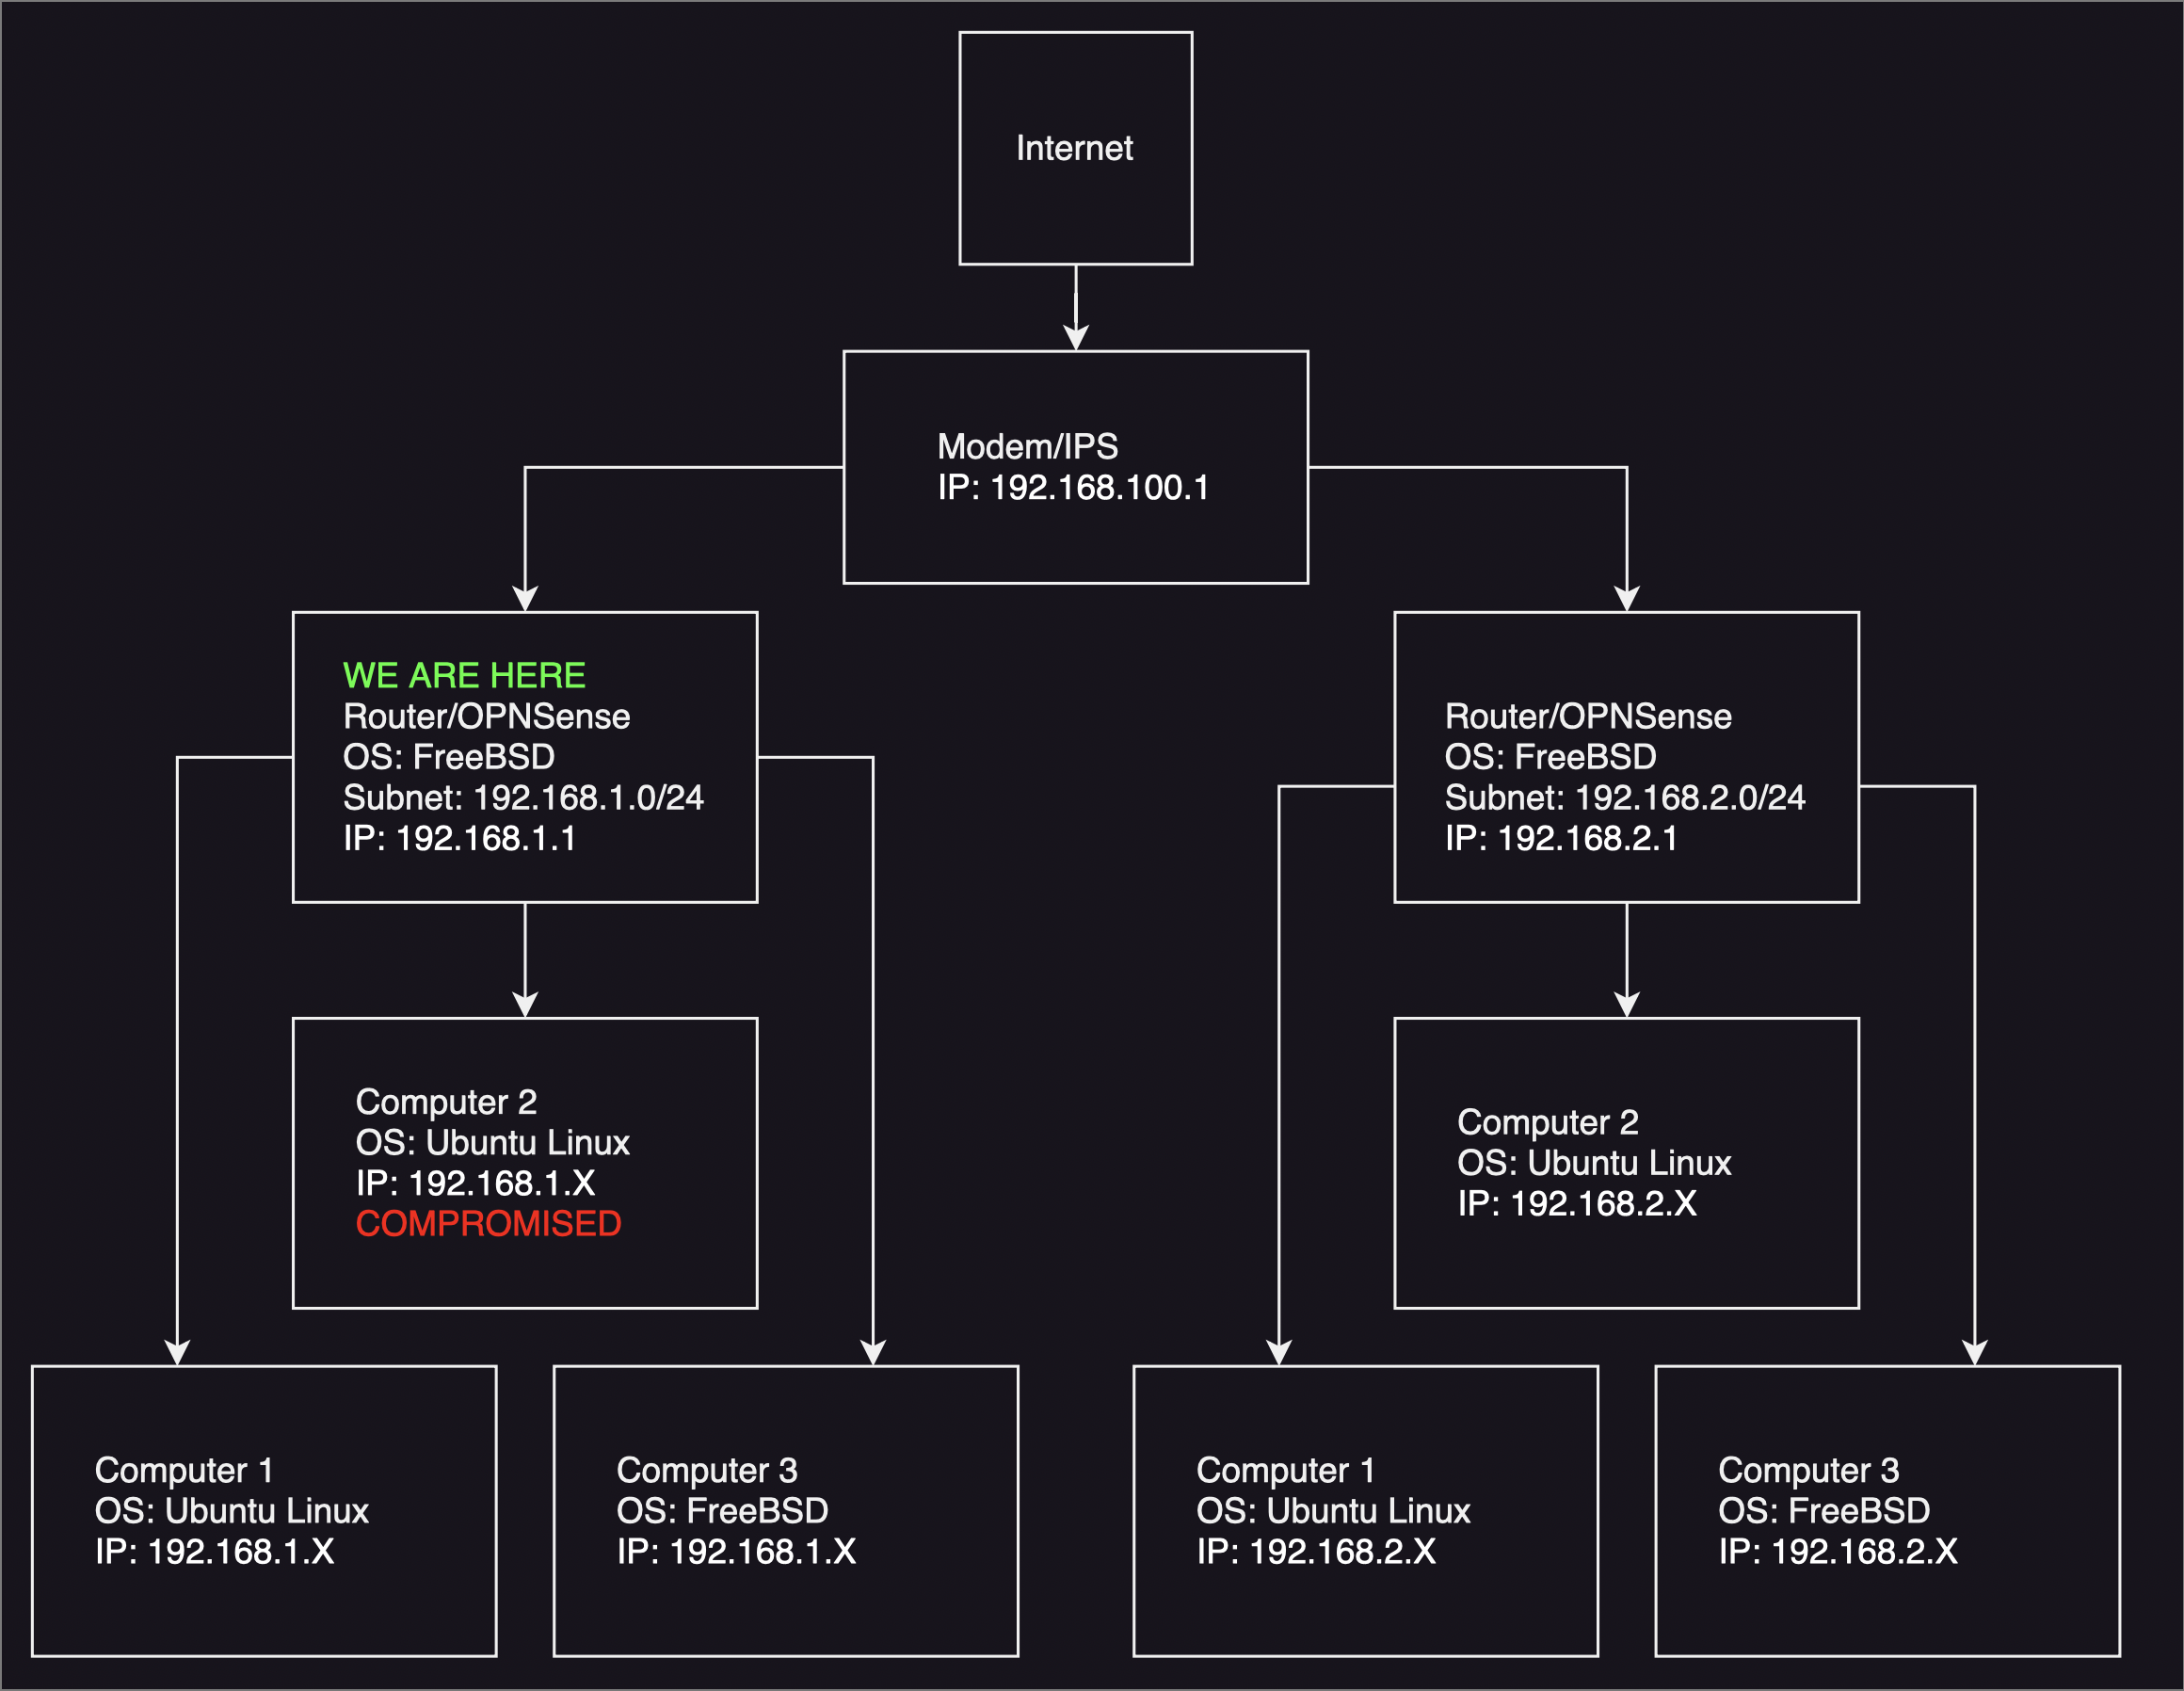
\includegraphics[width=0.5\textwidth]{diagram.png}
   \label{fig:network-topology}
\end{figure}

%-------------------------------------------------------------------------------

Our threat model concerns the scenario in which a system is attacked. Specifically, we focus on the scenario depicted in Figure~\ref{fig:network-topology}, where three interconnected computers form a subnet, with one of these computers compromised. Within this context, our threat model revolves around an attacker who has successfully gained access to one of the systems, as illustrated in the diagram. Once inside the network, the attacker's assumed objective is to scan other systems to identify vulnerabilities for lateral movement. The provided script, named ip-shuffle, plays a crucial role in this threat model, as it allows for the dynamic assignment of random IP addresses to network interfaces. The attackers' assumed capabilities are that they have basic user access to the compromised system, can perform network reconnaissance via scanning the network, and system persistence. 


%-------------------------------------------------------------------------------
\section{System Design}

The IP-shuffle script offers a systematic approach to dynamic IP address assignment for network interfaces in Linux and FreeBSD environments. Built around Bash scripting, it seamlessly orchestrates the IP address allocation process. By default, the program runs every 3 minutes, based on the provided cronjob. During execution, the script dynamically configures the IP address, gateway, network interface details, and other parameters, providing a flexible framework for network configuration. Through dedicated functions such as
\begin{verbatim}
generate_random_ip (), 
check_ip_availability(), 
and validate_network_config(), 
\end{verbatim}
the script ensures that the assigned IP addresses are compatible with the network infrastructure. It also incorporates error-trapping mechanisms and support for common Unix signals to enhance reliability and resilience, safeguarding against potential errors or interruptions. The script's flexibility is maintained through adherence to modular design principles, allowing seamless adaptation to diverse network configurations and environments. However, since the IP addresses are not persistent after a reboot for DHCP-configured machines, the script includes functions like \texttt{reset\_network()} for error recovery. The IP-shuffle script encapsulates a robust solution for automating network interface configuration tasks, embodying a sophisticated yet accessible approach to dynamic IP address management.
 
%-------------------------------------------------------------------------------
%-------------------------------------------------------------------------------
\section{Evaluation}

This is our evaluation.

%-------------------------------------------------------------------------------
%-------------------------------------------------------------------------------
\section{Conclusion}

MTD is proposed as one of the "game-changing" themes in cyber security.
Its vision is described as follows: create, evaluate, and deploy mechanisms
and strategies which are diverse, continually shifting and change over time
to increase complexity and costs for attackers, limit the exposure of vulnerabilites
and opportunities for attack, and increase system resiliency~\cite{cai2016introduction}.
IT WORKED!!!
The ip-shuffle script presents a robust solution for dynamically allocating random IP 
addresses to network interfaces, a critical element of network security strategies aimed 
at deterring potential attackers. Through the use of Bash scripting, it provides functionalities 
for generating IP addresses, checking availability, and validating network configurations, 
ensuring efficient and reliable IP address assignment. Its error handling capabilities and 
responsiveness to Unix signals improve reliability during execution, strengthening network 
resilience against errors or disruptions. Additionally, its modular design allows for easy 
adaptation to different network setups and environments, making it a valuable tool for 
automating tasks related to network interface configuration. Moreover, ip-shuffle embodies 
the concept of IP shuffling, a technique designed to complicate attackers' reconnaissance efforts 
by constantly changing IP addresses in an unpredictable manner. By assigning random IP addresses
dynamically, ip-shuffle contributes to organizations' proactive defense stance, increasing the 
difficulty for attackers to identify and exploit vulnerabilities. In essence, ip-shuffle represents 
a sophisticated yet user-friendly approach to managing dynamic IP addresses, empowering organizations 
to enhance their overall security posture and mitigate the impact of cyber threats.

%-------------------------------------------------------------------------------
\bibliographystyle{plain}
\bibliography{refs}

%%%%%%%%%%%%%%%%%%%%%%%%%%%%%%%%%%%%%%%%%%%%%%%%%%%%%%%%%%%%%%%%%%%%%%%%%%%%%%%%
\end{document}
%%%%%%%%%%%%%%%%%%%%%%%%%%%%%%%%%%%%%%%%%%%%%%%%%%%%%%%%%%%%%%%%%%%%%%%%%%%%%%%%

%%  LocalWords:  endnotes includegraphics fread ptr nobj noindent
%%  LocalWords:  pdflatex acks
